\chapter{СХЕМА СИСТЕМЫ МОНИТОРИНГА И ВЫБОР КОМПОНЕНТОВ КОНТРОЛЛЕРА}

\section{Общая структура схемы системы мониторинга электроэнергии}

Схема дистанционного мониторинга состоит из двух частей, взаимодействующих между собой: ИИК (Информационно-измерительный канал) и ИВК (Информационно-вычислительный комплекс). ИВК можно условно разделить на два уровня - нижний и верхний. Нижний уровень уровень включает в себя:
\begin{enumerate}
	\item устройства сбора и передачи данных (УСПД);
	\item каналы связи между электросчетчиками и УСПД;
	\item контроллеры удаленного сбора данных (КУСД);
	\item коммуникационная среда и каналы связи между КУСД и серверами верхнего уровня;
\end{enumerate}

Верхний уровень включает в себя:
\begin{enumerate}
	\item серверы верхнего уровня;
	\item ПО верхнего уровня;
	\item автоматизированные рабочие места(АРМ) диспетчеров и т.д;
\end{enumerate}

В данной системе удаленного мониторинга, Устройство Сбора и Передачи Данных (УСПД) --- это счетчик электрической энергии <<Меркурий 230ART-03>>. Разрабатываемый контроллер в системе АСКУЭ выполняет функции Контроллера Удаленного Сбора Данных (КУСД). Канал связи нижнего уровня представлен шиной CAN, а коммуникационная среда между КУСД и сервером (канал связи верхнего уровня) представлена глобальной компьютерной сетью Интернет либо Локальной Вычислительной Сетью (ЛВС) на базе различных технологий (например Ethernet). К каналу связи нижнего уровня можно подключать до 240 счетчиков к одному контроллеру\cite{mercinfo1}. Удаленным сервером в АСКУЭ является компьютер, на котором имеется программа, обеспечивающая взаимодействие с КУСД. В данной работе предусматривается разработка ПО только для КУСД.

Схема системы мониторинга отображена на рисунке \ref{fig:ascaepscheme}.

\begin{figure}[h!]
	\centering
		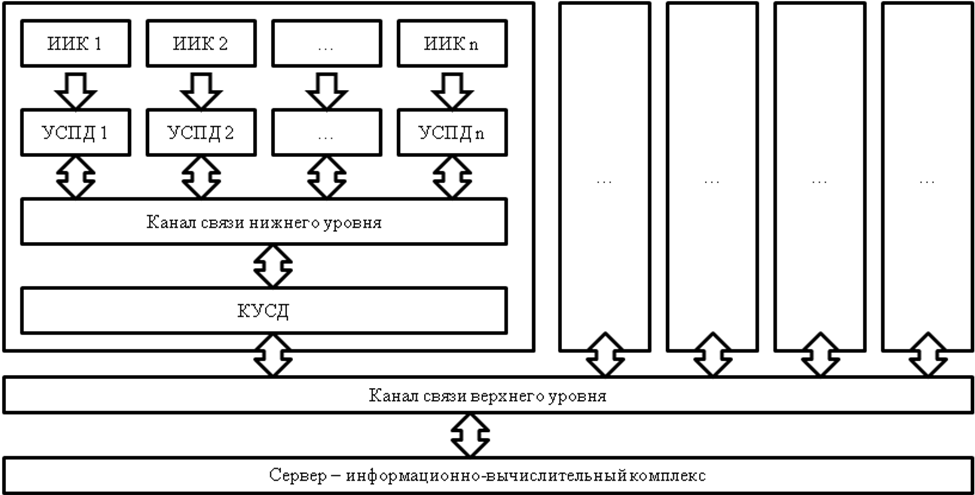
\includegraphics[scale=1.0]{img/ascaepscheme.png}
	\caption{Схема системы мониторинга электрической энергии \label{fig:ascaepscheme}}
\end{figure}

\section{Структурная схема разрабатываемого контроллера}

Связка КУСД и УСПД отображена на рисунке \ref{fig:controllerandmercury}.

\begin{figure}[h!]
	\centering
		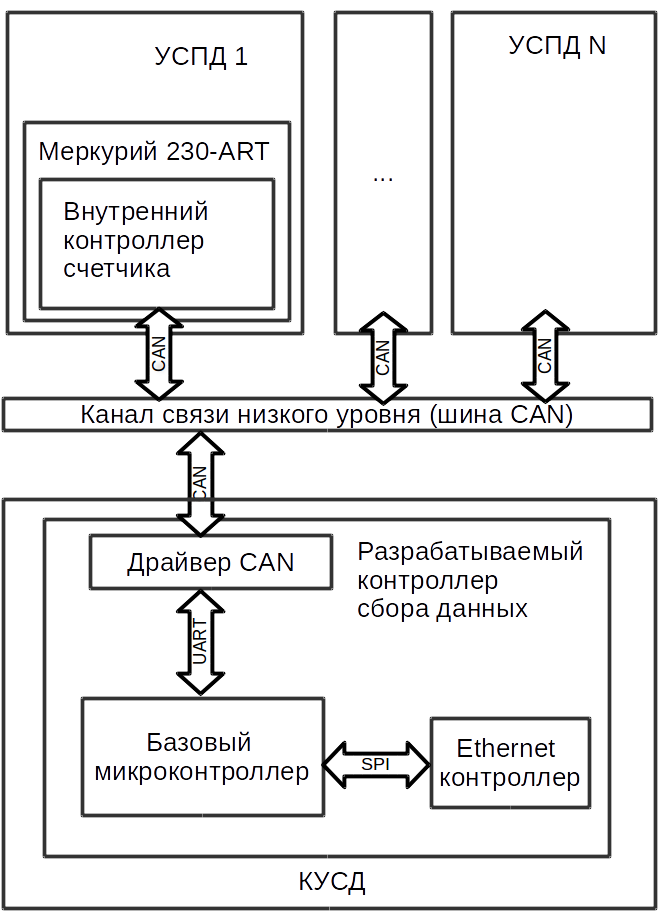
\includegraphics[scale=0.5]{img/controller_mercury.png}
	\caption{Схема системы мониторинга электрической энергии \label{fig:controllerandmercury}}
\end{figure}

Из рисунка можно выделить три основных блока КУСД:
\begin{enumerate}
	\item драйвер шины CAN;
	\item базовый микроконтроллер;
	\item Ethernet контроллер;
\end{enumerate}

\section{Программное обеспечение системы}

Программное обеспечение системы включает в себя:

\begin{enumerate}
	\item программное обеспечение КУСД и УСПД (прошивка);
	\item протокол связи между УСПД и КУСД, а также между КУСД и сервером системы;
	\item серверное программное обеспечение:
	\begin{enumerate}
		\item операционная система сервера;
		\item базы данных системы;
		\item реляционная СУБД;
		\item модуль взаимодействия с КУСПД;
	\end{enumerate}
	\item программное обеспечение пользователя системы (клиентское ПО);
\end{enumerate}

\section{Выбор компонентов контроллера}

\subsection{Базовый микроконтроллер}

Базовый микроконтроллер является основой КУСД. Перечень необходимых требований предъявляемых к микроконтроллеру:
\begin{itemize}
	\item наличие Flash-памяти программ с большим числом циклов записи;
	\item наличие энергонезависимой репрограммируемой памяти для хранения конфигурации (например EEPROM);
	\item наличие интерфейсов и портов ввода/вывода для подключения периферийных устройств:
	\begin{itemize}
		\item[•] интерфейс USART (UART) для взаимодействия с драйвером CAN, а также настроек конфигурации;
		\item[•] интерфейс SPI для сопряжения с Ethernet контроллером;
	\end{itemize}
	\item доступная цена;
	\item приемлемая для функционирования системы производительность;
	\item доступность в свободной продаже на отечественном рынке;
\end{itemize}

В соответствии с перечисленными требованиями был выбран 8-разрядный микроконтроллер ATmega328/P фирмы Atmel. Этот микроконтроллер имеет достаточную производительность, широко доступен на рынке (по состоянию на 2017 г.) по приемлемой цене и потребляет малый ток в активном режиме.

К его отличительным особенностям можно отнести\cite{atmegainfo}:
\begin{itemize}
	\item продвинутая RISC архитектура:
	\begin{itemize}
		\item[•] 131 исполняемых команд;
		\item[•] 32 рабочих регистра общего назначения;
		\item[•] полностью статический режим работы;
		\item[•] большинстов команд выполняются за один машинный такт;
		\item[•] встроенный 2-х тактовый умножитель;
	\end{itemize}
	\item износостойка и энергонезависимая память программ и данных:
	\begin{itemize}
		\item[•] 32 Кбайт репрограммируемой Flash памяти для команд;
		\item[•] 1 Кбайт EEPROM;
		\item[•] 2 Кбайт внутренней SRAM;
		\item[•] программируемый ключ для защиты прошивки;
		\item[•] срок сохранения данных: 20 лет при температуре 85 $^{\circ}$C и 100 лет при температуре 25 $^{\circ}$C;
	\end{itemize}
	\item периферийные функции:
	\begin{itemize}
		\item[•] два 8-битных таймера/счётчика с программируемым предделителем и режимом сравнения;
		\item[•] один 16-битный таймер/счетчик с программируемым предделителем, режимом сравнения и режимом захвата;
		\item[•] счётчик реального времени с программируемым генератором;
		\item[•] 6 ШИМ генераторов;
		\item[•] два 10-битных АЦП;
		\item[•] два Master/Slave SPI последовательных интерфейса;
		\item[•] один программируемый последовательный USART интерфейс;
		\item[•] программируемый Watchdog таймер с программируемым генератором;
		\item[•] встроенный аналоговый компаратор;
		\item[•] прерывания и уход из спящего режима по изменению уровня на ножке;
	\end{itemize}
	\item 23 программируемых линии ввода/вывода;
	\item напряжение питания: 1,8-5,5 В;
	\item рабочий температурный диапазон: от -40$^{\circ}$C до 105$^{\circ}$C;
	\item энергопотребление при частоте 1МГц, 1,8В, 25$^{\circ}$C:
	\begin{itemize}
		\item[•] активный режим: 0,2 мА;
		\item[•] режим энергосбережения: 0,75 мкА;
		\item[•] режим выключенного питания: 0,1 мкА;
	\end{itemize}
\end{itemize}

Для данной работы в качестве макетного образца для испытания работы сетевых протоколов будет использована готовая плата контроллера Arduino UNO R3. Внешний вид платы отображен на рисунке \ref{fig:arduino}.

\begin{figure}[h!]
	\centering
		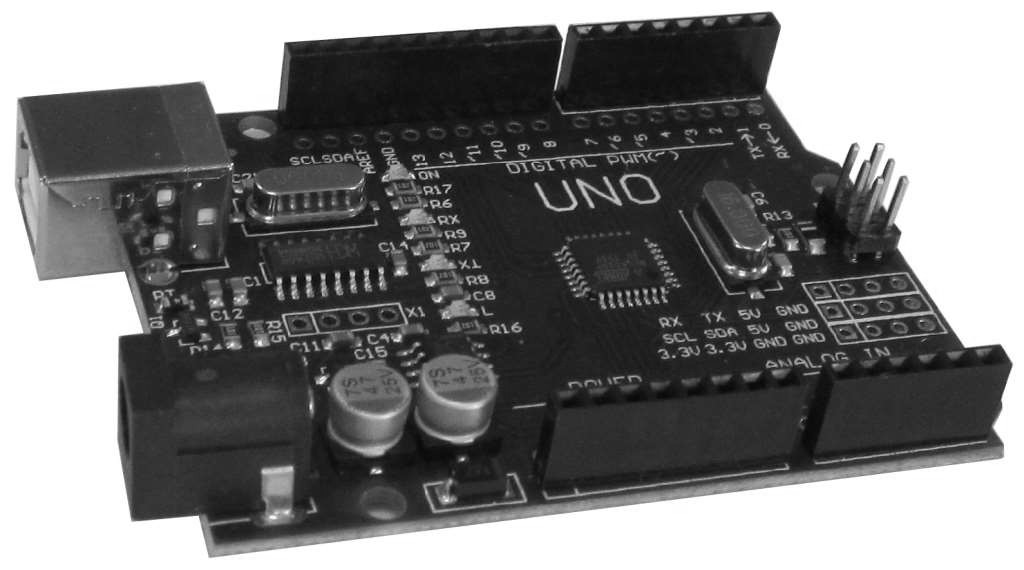
\includegraphics[scale=0.56]{img/arduino_uno_r3.jpg}
	\caption{Внешний вид платы Arduino UNO R3\label{fig:arduino}}
\end{figure}

Данная плата произведена на базе микроконтроллера ATmega328/P с тактовой частотой 16 МГц. Особенности данной платы\cite{arduino}:
\begin{itemize}
	\item питание:
	\begin{itemize}
		\item[•] может питаться как от USB подключения, так и от внешнего источника: батарейки или обычной электрической сети;
		\item[•] работает при наличии напряжения от 6 до 20 В, однако при напряжении менее 7 В работа может быть неустойчивой, а напряжение более 12 В может привести к перегреву и повреждению;
	\end{itemize}
	\item память: из 32 Кбайт Flash-памяти ATmega328/P 2 Кбайт отведено под так называемый \textit{bootloader}. Он позволяет прошивать контроллер с использованием последовательного UART интерфейса, а используя встроенный переходник USB <-> COM TTL (RS232) CH340G можно прошивать контроллер используя USB.
	\item защита USB: плата обладает предохранителем, защищающим USB-порты от перенапряжения и коротких замыканий;
	\item габариты: размер платы составляет 6,9 x 5,3 см;
\end{itemize}

\subsection{Ethernet контроллер ENC28J60}

ENC28J60 ~--- это Ethernet микроконтроллер с SPI интерфейсом. Он удовлетворяет всем спецификациям стандарта IEEE 802.3. Микросхема реализует сервисы физического уровня и MAC-подуровня канального уровня в модели OSI. На физическом уровне действует спецификация 10BASE-T PHY. Полностью совместима с 10/100/1000Base-T. Внешний вид микросхемы изображен на рисунке \ref{fig:enc28j60}.

Технические характеристики\cite{enc28j60datasheet}:
\begin{itemize}
	\item поддержка полнодуплексного и полудуплексного режима;
	\item имеет программируемую настройку рассчёта CRC и заполнения кадра;
	\item имеет SPI интерфейс со скоростью обмена не более 20 МГц;
	\item встроенный DMA для быстрого перемещения данных;
	\item буфер входящих пакетов является аппаратно-управляемым циклическим FIFO буфером;
	\item поддержка Unicast, Multicast и Broadcast пакетов;
	\item имеет программируемую настойку фильтрации входящих пакетов;
	\item имеет шесть источников прерываний и один вывод для внешнего прерывания;
	\item напряжения питания 3,1-3,6 В;
	\item входы толерантны к 5 В;
	\item температурный диапазон:  от -40 до +85 $^{\circ}$C.
\end{itemize}

В разрабатываемом контроллере используется готовый Ethernet модуль на базе ENC28J60. Данный модуль имеет всю необходимую для работы периферию:
\begin{itemize}
	\item <<розетка>> физического сетевого интерфейса Rj-45;
	\item кварц 25 МГц;
	\item светодиоды состояния;
	\item выводы SPI интерфейса;
	\item выводы для подключения питания 3,3/5 В;
	\item стабилизатор напряжения на 3,3 В;
\end{itemize}

Внешний вид модуля изображен на рисунке \ref{fig:ethcontroller}.

\begin{figure}[h!]
	\centering
		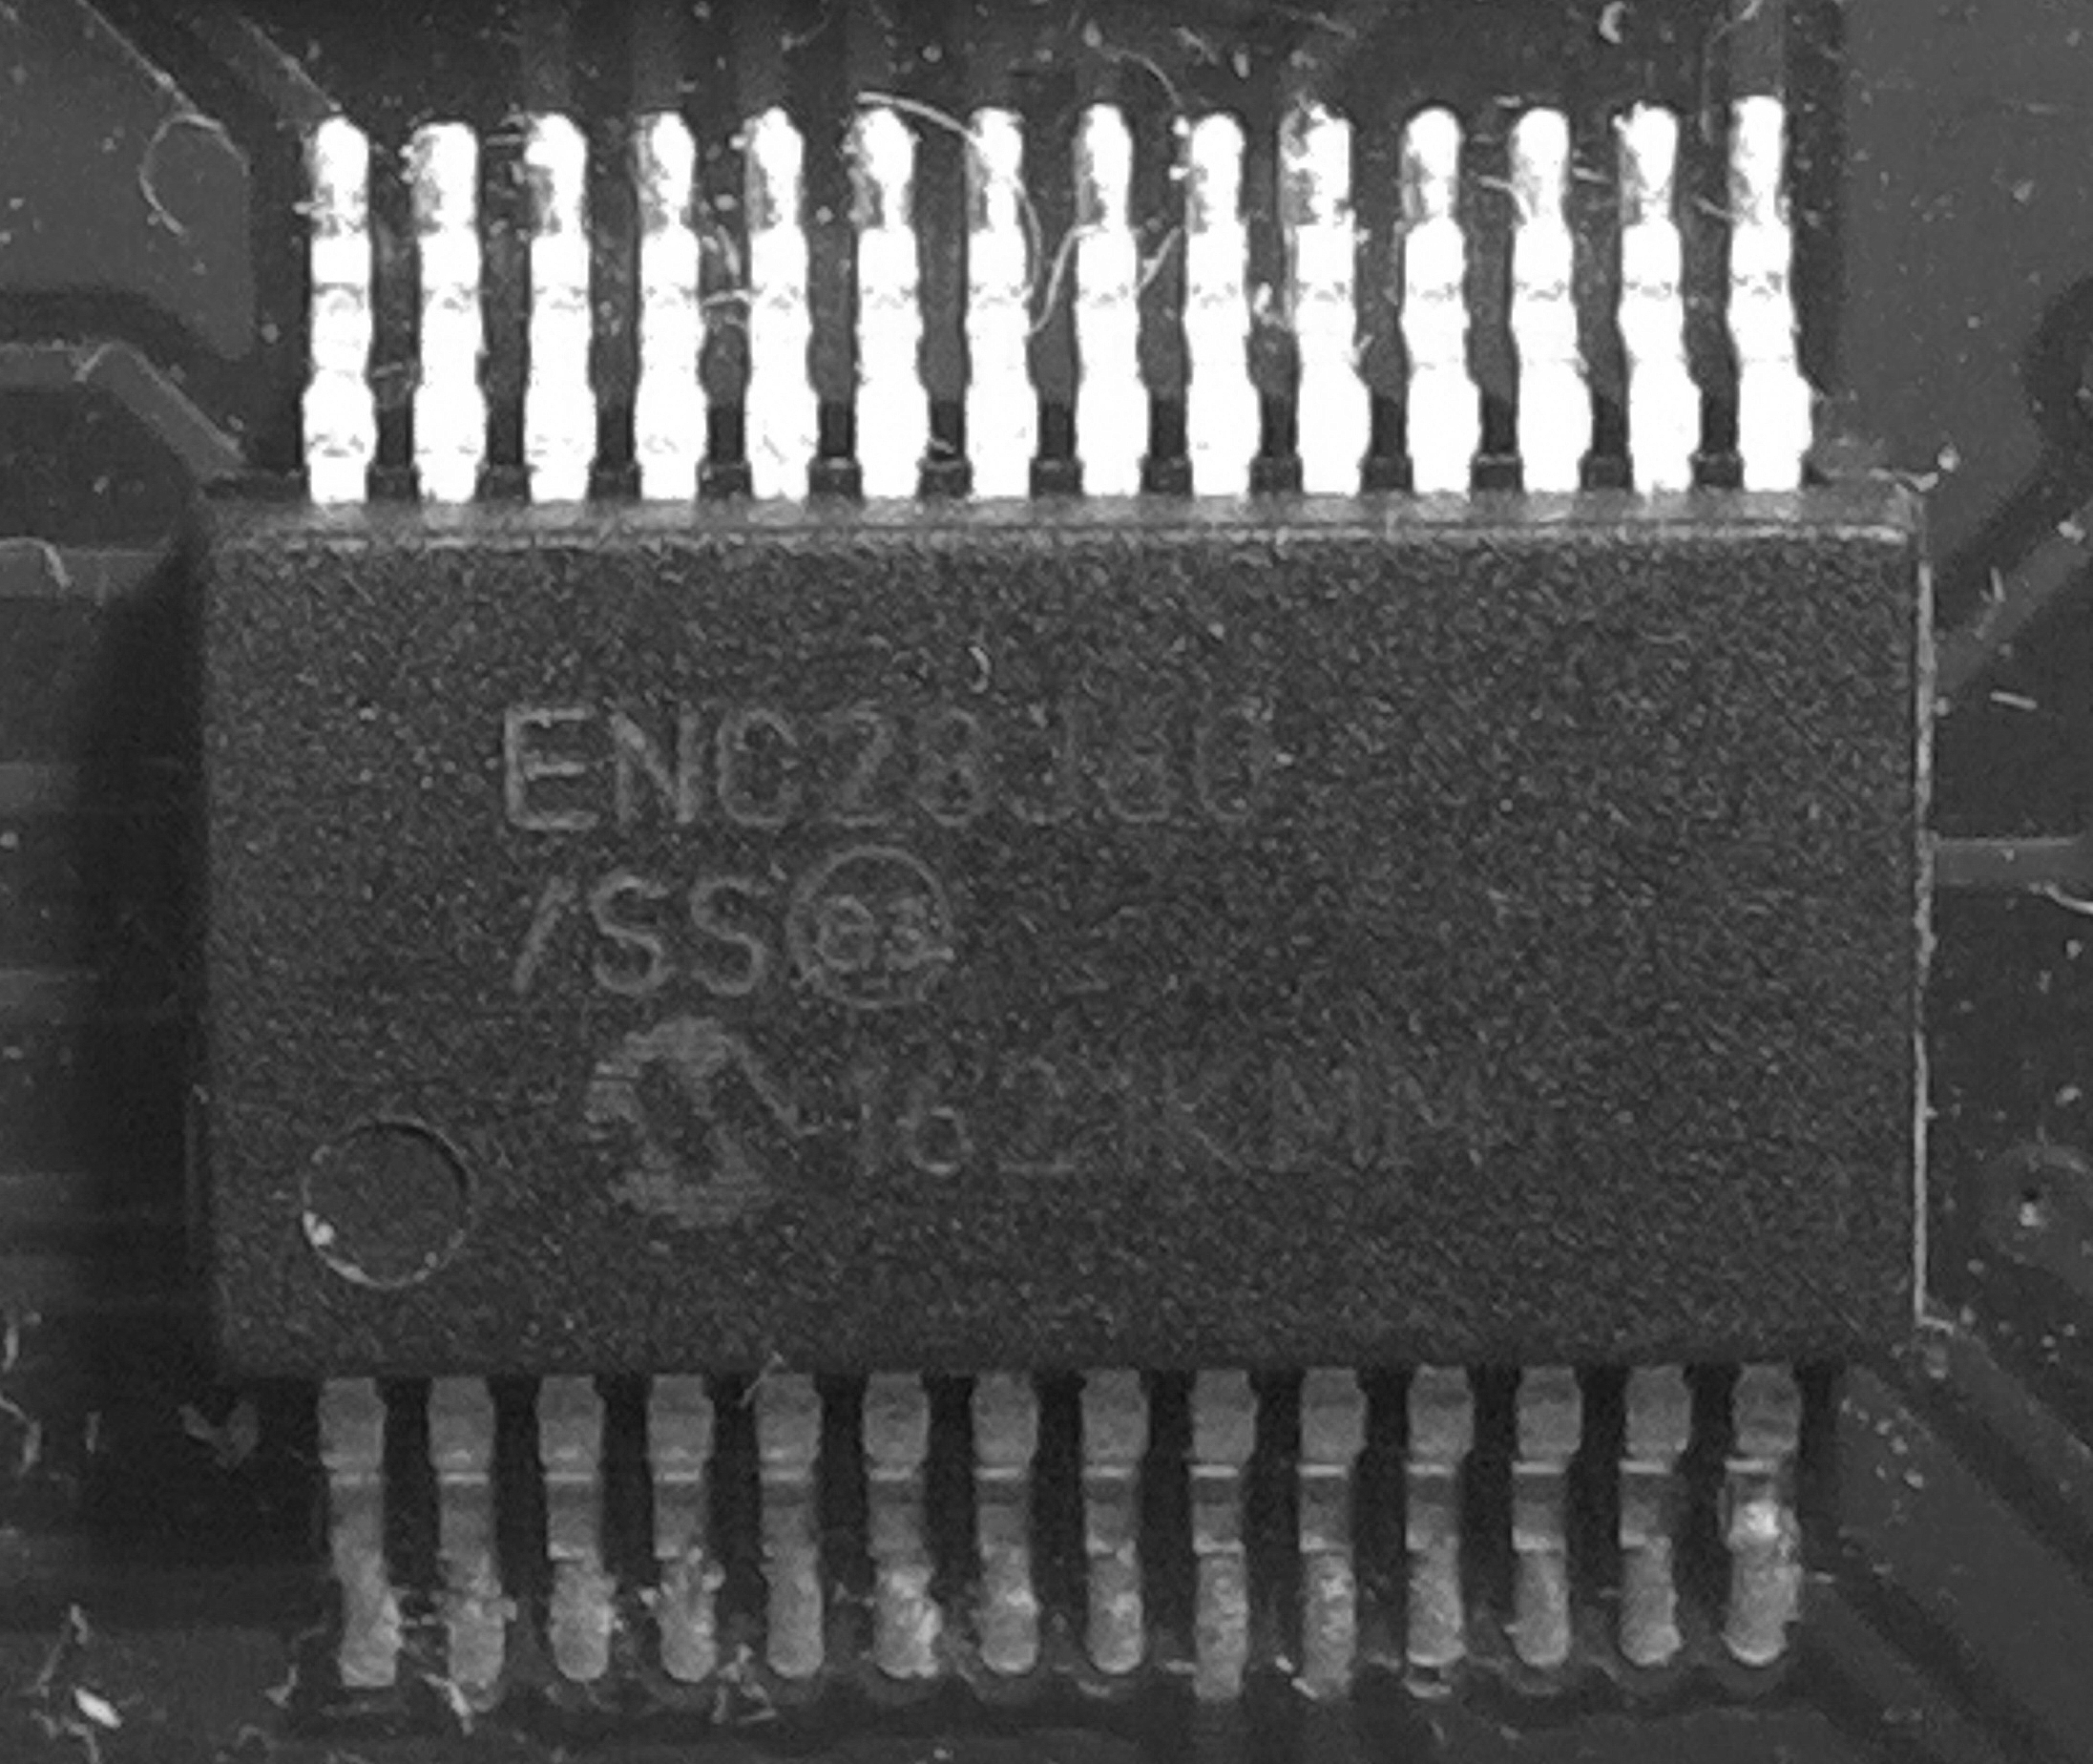
\includegraphics[scale=0.09]{img/enc28j60.png}
		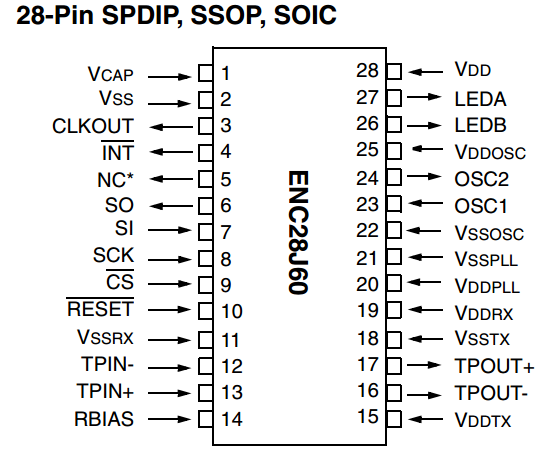
\includegraphics[scale=0.36]{img/enc28j60io.png}
	\caption{Внешний вид микросхемы ENC28J60 и расположение выводов\label{fig:enc28j60}}
\end{figure}


\begin{figure}[h!]
	\centering
		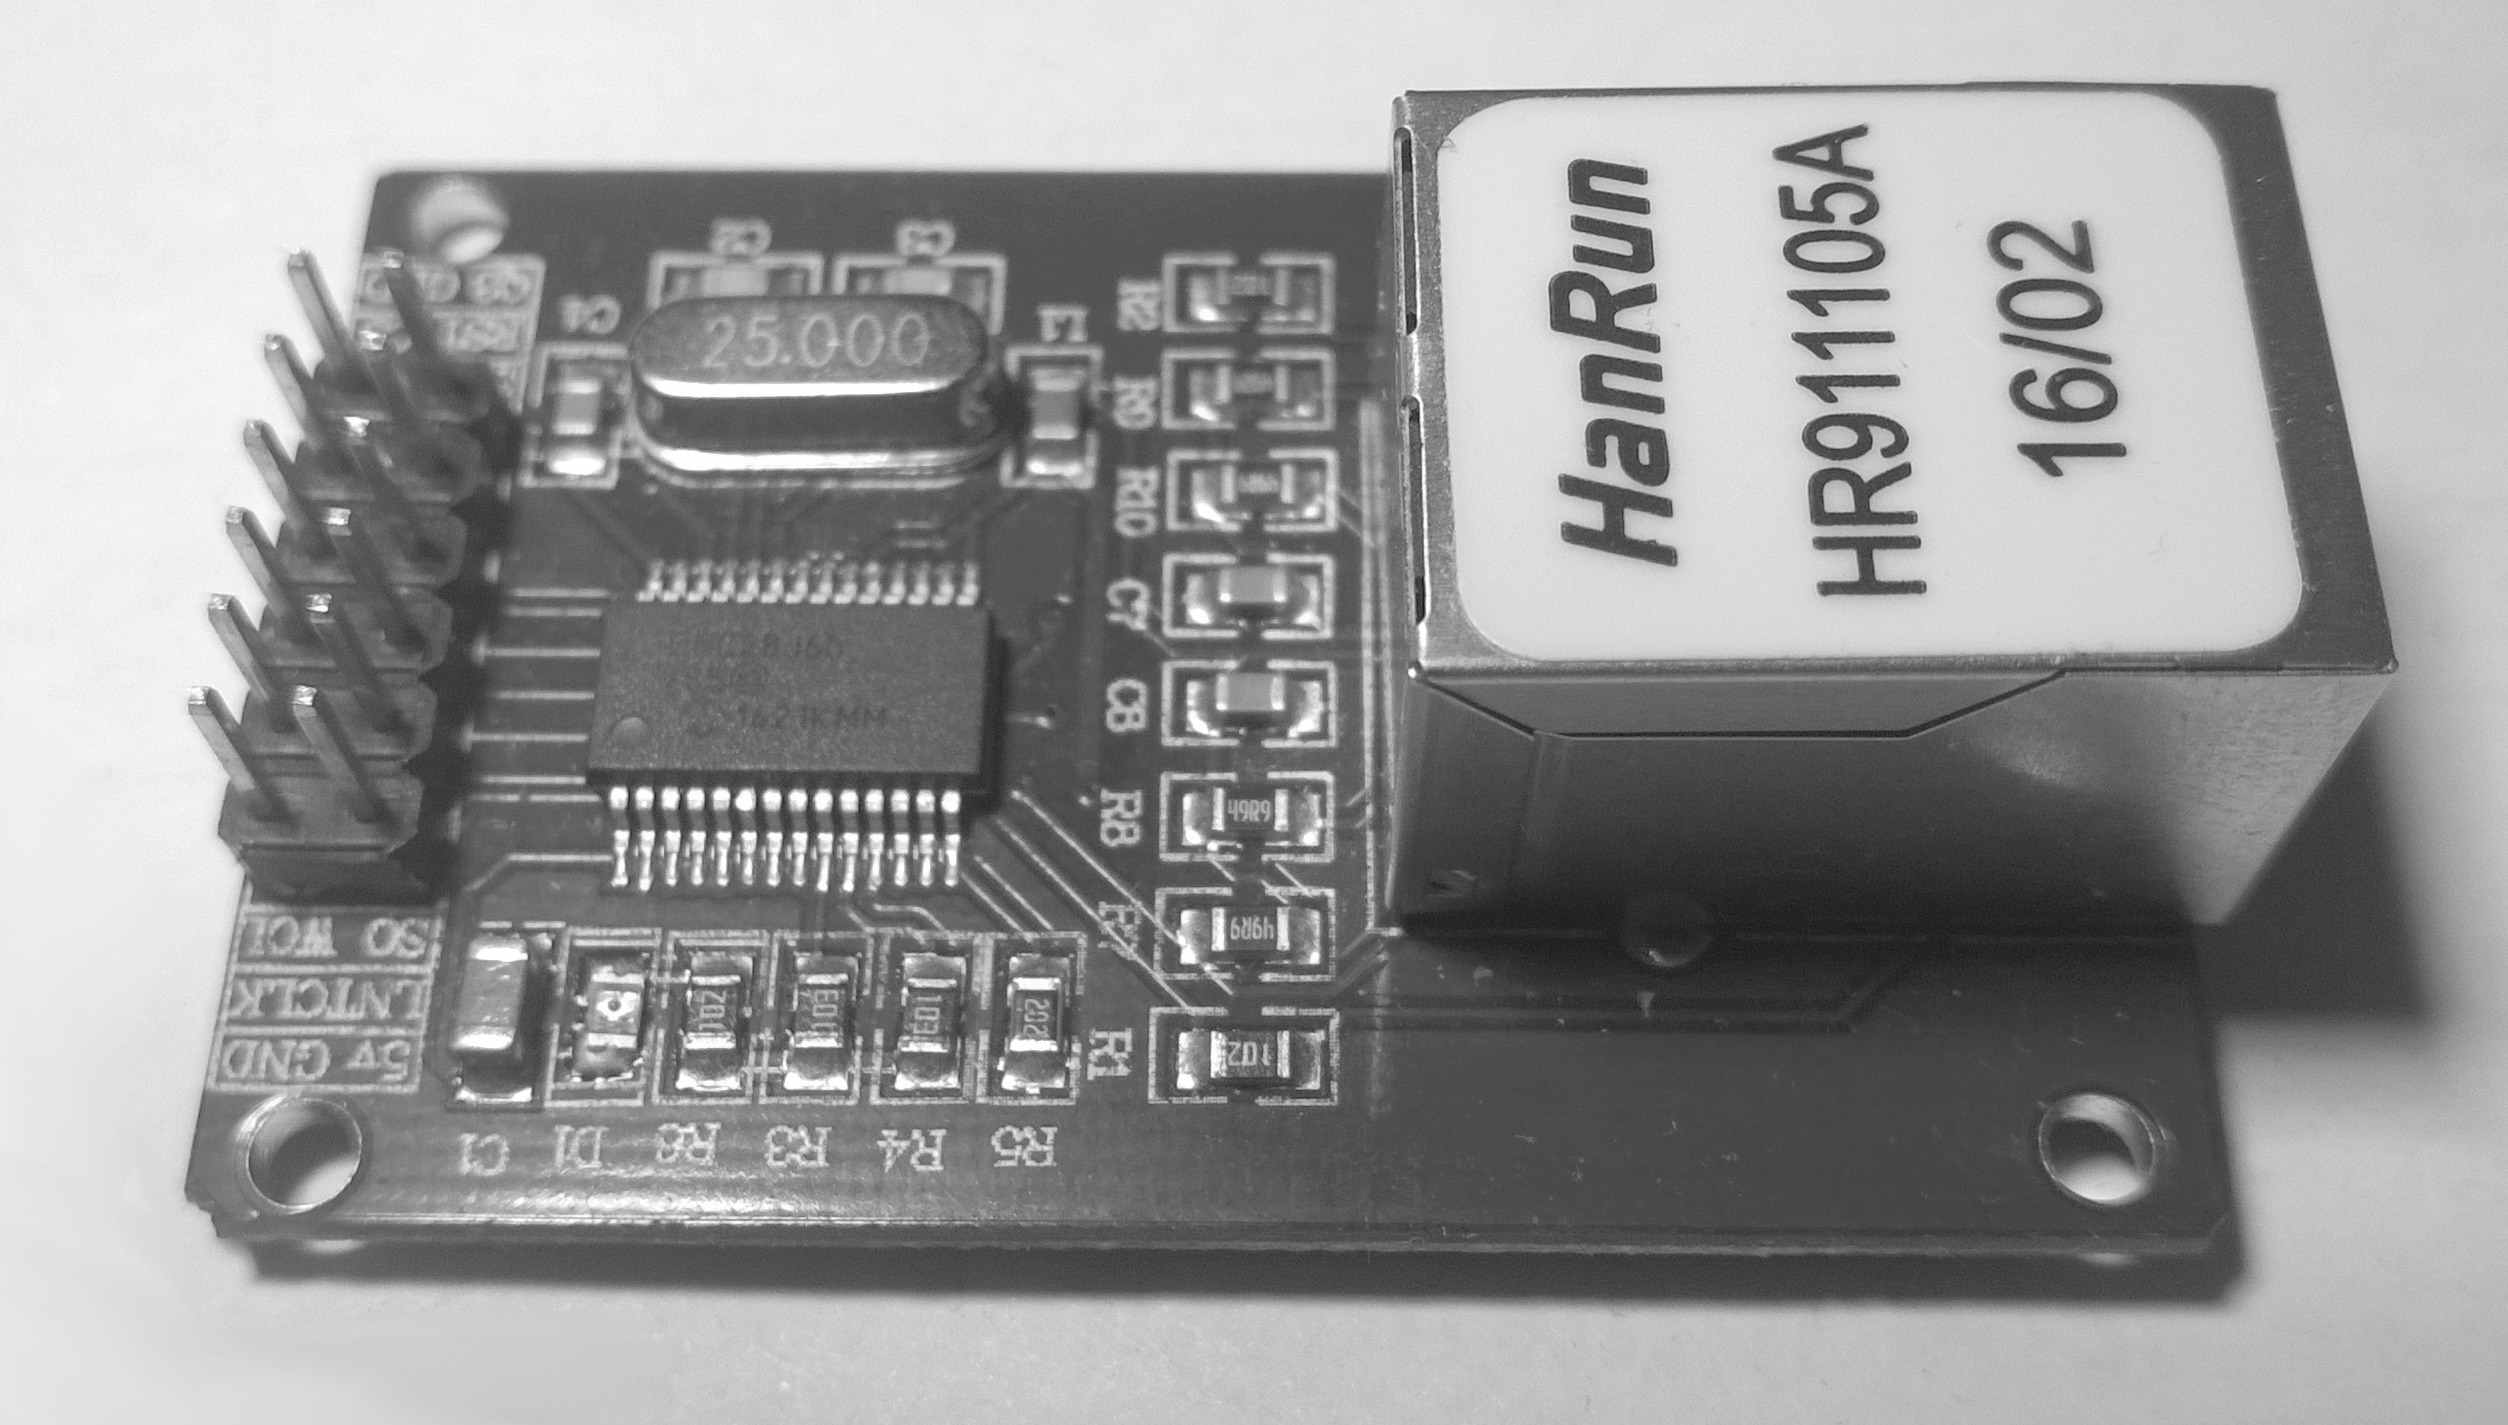
\includegraphics[scale=0.1]{img/ethcontroller.png}
		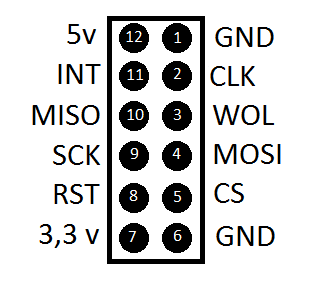
\includegraphics[scale=0.5]{img/ethpins.png}
	\caption{Внешний вид модуля и расположение выводов для подключения к КУСД\label{fig:ethcontroller}}
\end{figure}

Типичная схема подключения ENC28J60 изображена на рисунке \ref{fig:typicalinterface}

\begin{figure}[H]
	\centering
		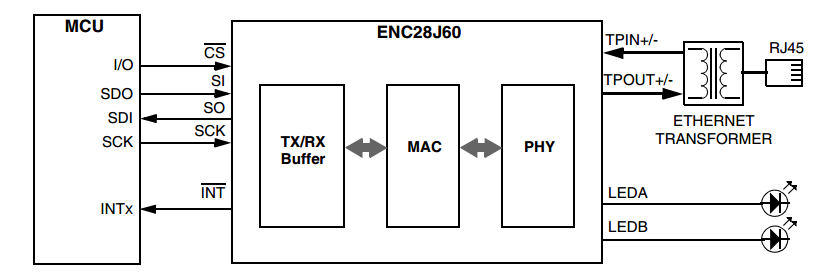
\includegraphics[scale=0.6]{img/typicalinterface.png}
	\caption{Типичное строение сетевого интерфейса на базе ENC28J60\label{fig:typicalinterface} \cite{enc28j60datasheet}}
\end{figure}

\subsubsection{Архитектура ENC28J60}

Основные блоки ENC28J60 отображены на рисунке \ref{fig:encblocks}.

\begin{figure}[H]
	\centering
		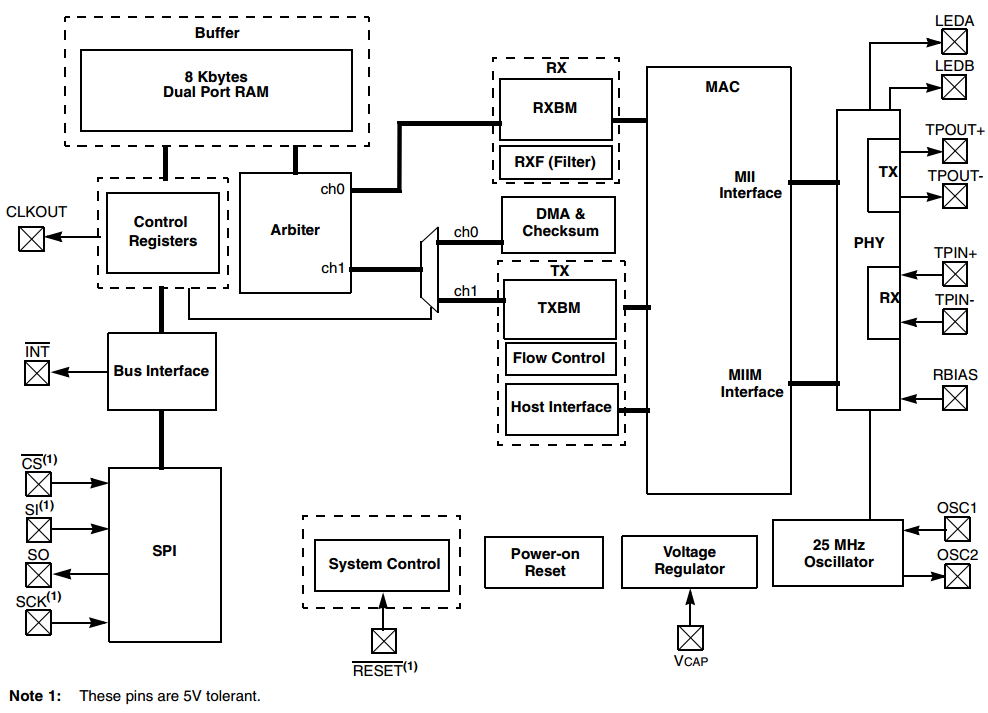
\includegraphics[scale=0.5]{img/encblockdiagram.png}
	\caption{Блок-диаграмма ENC28J60\label{fig:encblocks} \cite{enc28j60datasheet}}
\end{figure}

\begin{itemize}
	\item PHY --- физический уровень. Приёмник, передатчик, драйверы и т.д. Все, что необходимо для работы с определенное средой передачи данных. В данном случае --- с витой парой, по стандарту 10BASE-T. ДОступ к PHY происходит исключительно через MII - Medium Independent Interface. PHY имеет свой набор 16-битных регистров, доступ к которым осуществляется через MII;
	\item MAC (Medium access Controller) --- канальный уровень. В него входит вся логика, необходимая для отправки и приема пакетов в сети Ethernet. MAC отвечает за адресацию, рассчёт контрольной суммы, фильтрацию принимаемых пакетов, разрешение коллизий и т.д;
	\item Управляющая логика отвечает за все остальное. В том числе, обслуживает буфер из которого MAC берет отправляемые данные и складывает принятые. Управляет режимами энергопотребления и т.д;
\end{itemize}

Вся память в ENC28J60 делится на буфер для данных, управляющие регистры и регистры PHY.

Управляющие регистры делятся на 4 банка. Каждый банк имеет размер в 32 регистра, но последие 5 адресов (0x1b..0x1f) адресуют общие регистры, вне зависимости от того, какой банк выбран. Полное описание управляющих регистров ENC28J60 можно увидеть на изображении \ref{fig:encregmap}. Управляющие регистры напряму доступны через интерфейс SPI. 

\begin{figure}[H]
	\centering
		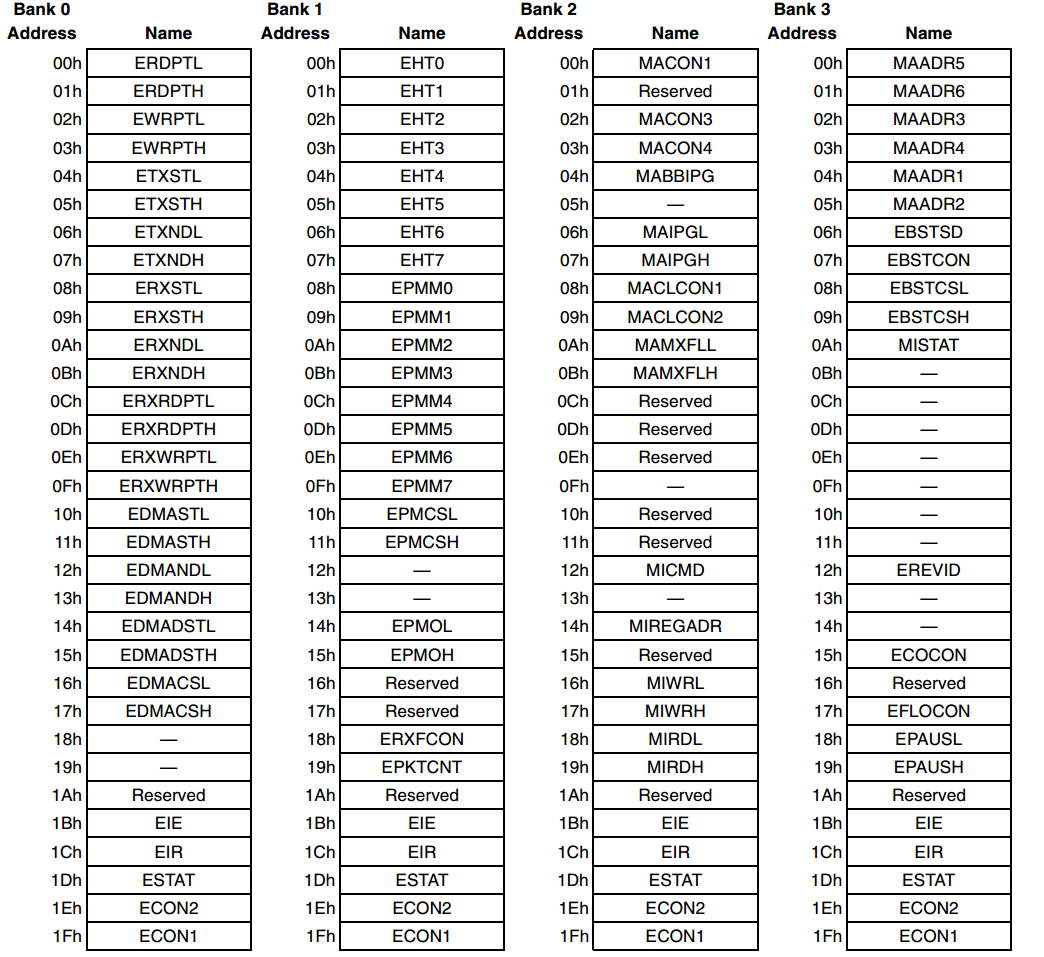
\includegraphics[scale=0.45]{img/encregmap.png}
	\caption{Управляющие регистры ENC28J60\label{fig:encregmap} \cite{enc28j60datasheet}}
\end{figure}

В ENC28J60 есть буфер размером 8 Кбайт. Часть этого буфера обычно выделяется для приёма пакетов, а часть - для передачи. В банке 0 управляющих регистров содержатся специализированные регистры для работы с данным буфером. Логика их работы позволяет организовать кольцевой FIFO (\textit{First In, First Out}) буфер для принимаемых пакетов. Организация данного буфера отображена на рисунке \ref{fig:encethbuff}.

\begin{figure}[H]
	\centering
		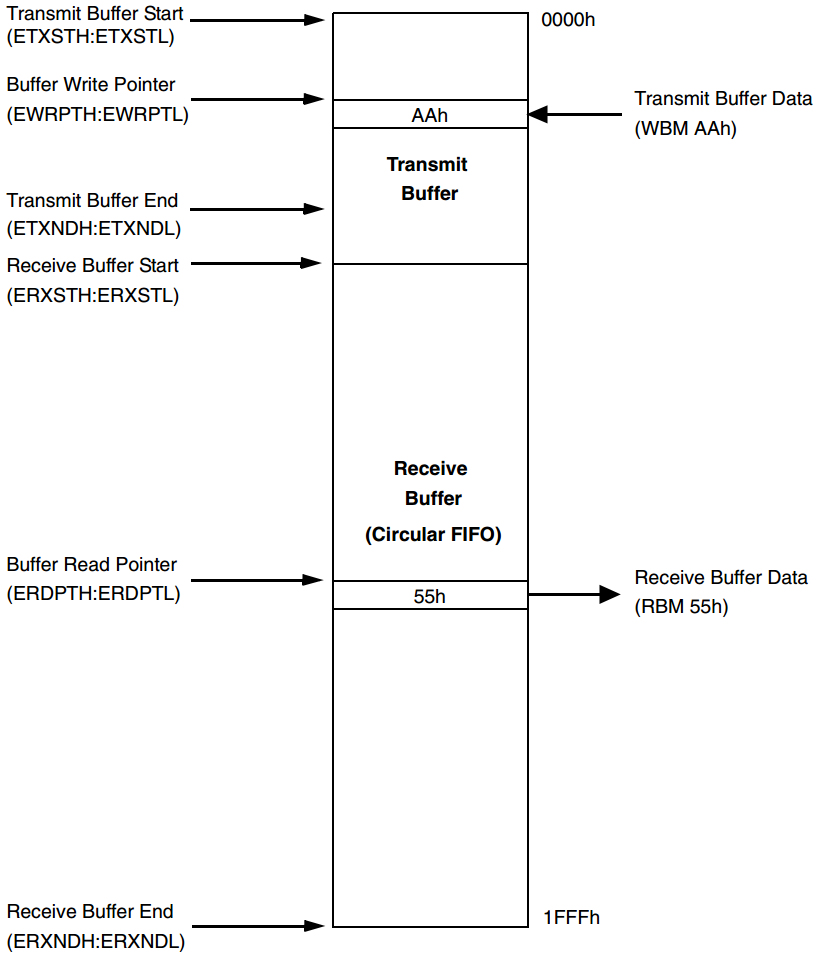
\includegraphics[scale=0.45]{img/encethbuff.png}
	\caption{Организация буфера принимаемых данных в ENC28J60\label{fig:encethbuff} \cite{enc28j60datasheet}}
\end{figure}




